%%================================================
%% Filename: chap02.tex
%% Encoding: UTF-8
%% Author: Yuan Xiaoshuai - yxshuai@gmail.com
%% Created: 2012-04-27 19:37
%% Last modified: 2019-11-05 23:57
%%================================================
\chapter{相关理论知识与关键技术}
\label{cha:basic-knowledge}
  
\section{源地址伪造攻击的分类}

源地址伪造攻击可以根据伪造产生的虚假地址与攻击者受害者所在网络的关系来进行分类,总共可分为六类:
a.虚假地址在网络中不存在或已经失活;
b.虚假地址指向的主机是受害者;
c.虚假地址与受害者主机处于同一个子网中;
d.虚假地址与攻击者处于同一个子网中;
e.虚假地址处于攻击者和受害者之间的路径中;
f.虚假地址既不在攻击者与受害者的子网中也不在攻击者与受害者之间的路径当中\onlinecite{Bi2010}。
以下是这六类攻击的详细描述,表~\ref{tab:source_address_spoofing}~展示了这六种攻击之间的关系。

\subsection*{a类}
 恶意主机通过产生随机的互联网中不存在的或着已经失效的IP地址来对攻击数据包的源地址进行伪造。
 产生的攻击数据包占用着受害者主机的资源,使受害者不能再向其他主机提供服务。
 这些IP地址包括RFC1918中指定的私有IP地址\cite{Rekhter1996}、RFC3330中的自动分配的IP地址\cite{BogonList2003}、循环测试地址,这些IP地址都不会在互联网中出现。
SYN Flood是一种常见的攻击方式,它能够不断消耗受害者主机CPU资源以及内存资源并阻止其他合法用户的连接。
在不设置保护策略的情况下,少量的SYN洪水攻击便足以使受害者主机崩溃。
由于受害者主机在受到攻击时会向恶意数据包中源地址指向的主机返回SYNACK包使其返回RTS包释放半连接。
这就导致了此种攻击的虚假地址将会采用上面所说的地址。
\subsection*{b类}
攻击者将受害者主机的IP地址作为攻击数据包的源地址以此来实现反射性攻击、直接攻击和诱捕攻击,这类攻击通常有三种形式:
攻击数据包的源地址是受害者主机IP地址,目标地址是受害者主机的所在子网的广播地址。
攻击数据包被广播之后,受害者将收到大量的ACK回复,这会使受害者淹没于这些流量当中而大大地削弱了受害者的正常服务能力。
攻击数据包的源地址与目标地址同时是受害者主机的IP,受害者收到攻击数据包后会将其响应发送给自己,这一行为会导致受害者受到干扰而瘫痪。
著名的DrDoS\cite{Gibson2002}是此类攻击的一个典型例子,它会使受害者的带宽或内存等资源溢出或者过载而不能使用。
TFN\cite{Dittrich1999}和Land  attacks\cite{CERT1997}也是此类典型的例子。
攻击者向受害者发送数据包,其源主机/端口与目标主机/端口相同,并设置了SYN标志能够锁死受害者或使其协议栈崩溃。
\subsection*{c类}
此类攻击将受害者所处子网中的IP地址作为攻击数据包中的源地址,并依赖于受害者和虚假地址所指向的主机之间的信任关系。
基于TCP连接的盲IP欺骗攻击\cite{Ali2007}是这类攻击的典型例子。
TFN2K\cite{Barlow2000}也是一个例子,它是TFN\cite{Dittrich1999}的下一代版本。
\subsection*{d类}
d类攻击将攻击者所处子网内的地址作为源地址,因为入口过滤的粒度通常不高便可以很容易使攻击数据包通过入口过滤。
反弹扫描\cite{CERT1997}是这类产品的一个典型例子,为了从受害者那里获取响应包,攻击者伪造同一子网络中邻居的源地址,并嗅探返回给邻居的流量数据。
这种攻击可用于端口扫描,如果受害者的一个端口被关闭,受害者将回复RST数据包\cite{Ray1981},更糟糕的是,这种攻击可以有效地逃脱uRPF的攻击\cite{CiscoIOS2005}。
\subsection*{e类}
攻击者通常强迫网络设备的源地址出现在攻击者与受害者之间的路径上。
在这种类型的攻击下,攻击者可以传播虚假的DNS或路由信息,并重定向网络流量\onlinecite{Huang2006}。这将被认为是最危险的袭击之一。
\subsection*{f类}
攻击者不依赖于受害者和虚假地址之间的特殊拓扑关系。
这类攻击通常被组合在一起,例如MITM攻击\cite{ManInTheMiddle2007}是两种典型的f类攻击的一种组合。
如A分别与V1和V2进行通信,则A在与V2通信时伪造V1的源地址,在与V1通信时伪造V2的源地址。

\begin{table}[htbp]
    \caption{源地址伪造攻击分类}
    \label{tab:source_address_spoofing}
    \centering
    \begin{tabular}{cccc}
    \toprule
    {\heiti 分类} & {\heiti 虚假地址状态} & {\heiti 与攻击者关系} & {\heiti 与受害者关系}  \\ 
    \midrule
    a类 & 不存在或已经失活 & 无 & 无 \\ 
    b类 & 存在 & 无 & 指向 \\ 
    c类 & 存在 & 无 & 同子网 \\ 
    d类 & 存在 & 同子网 & 无 \\ 
    e类 & 存在 & 攻击者到受害路径内 & 攻击者到受害者路径内 \\ 
    f类 & 不存在 & 无 & 无 \\ 
    \bottomrule
    \end{tabular}
    \end{table}

\section{数据包标记法}
图~\ref{fig:simple_topology}~是一个IP回溯问题的简单网络拓扑图。
整个结构可以看作是一棵以$V$为根节点的树,$V$代表一个遭受攻击的\textbf{受害者},它可能为服务器、防火墙或者入侵检测系统。
每个$A_i$是树中的叶子节点,它代表潜在的\textbf{攻击源},它可能为例如攻击者主机也可能为普通的用户。
每个$R_i$则代表从这些$A_i$到$V$的中间路由器。
在这个网络中,每个$A_i$都有可能向$V$发送数据包,而这些数据包中则有潜在攻击数据包的可能性。
其中这些攻击数据包走过的路径都为\textbf{攻击路径},它是一个从攻击节点$A_i$到$V$的有序唯一路由序列。
例如,假设$A_1$是一个攻击节点,它正在向$V$发送攻击数据包,这些攻击数据包走过的路径是唯一的,由$R_7$、$R_4$、$R_2$、$R_1$依次组成,则这条从$A_1$到$V$的唯一的路径就是一条攻击路径。
一个\textbf{IP回溯问题}就是通过一些方法和策略确定攻击路径,揭示攻击主机的真实身份和具体位置。

\begin{figure}[htbp]
    \centering
    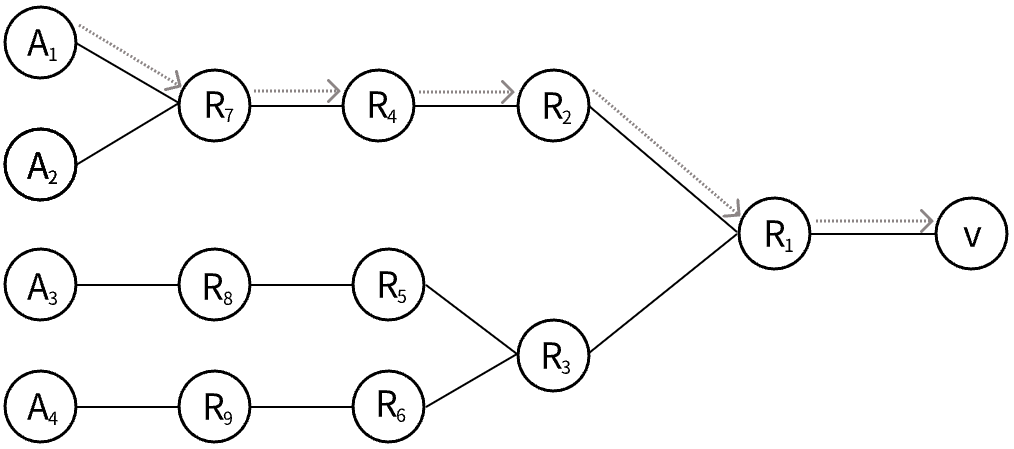
\includegraphics[width = 0.8\textwidth]{simple_topology.png}
    \caption{针对路由回溯问题的简单拓扑图}
    \label{fig:simple_topology}
  \end{figure}

当回溯成功后便可以从攻击源的下游最近邻路由器过滤掉这些数据包以保护受害者服务器免受攻击。
在这个问题中,似乎只要从攻击数据包中提取出源IP就可以确定攻击路径,然而解决这个问题通常是很复杂的。
一个有预谋、有准备的攻击通常会做出一些手段,例如伪造攻击数据包的源IP地址、发送一些虚假信息来伪造攻击路径从而干扰溯源,使溯源任务极难完成。



一个IP回溯问题相对简单的近似溯源为找到一条包含有真实攻击路径作为路径后缀的候选路径,这个路径后缀就是有效后缀\cite{savage2000practical}。
例如,$R_8$、$R_5$、$R_3$、$R_7$、$R_4$、$R_2$、$R_1$就是一条有效的候选路径,因为它包含$R_7$、$R_4$、$R_2$、$R_1$这条真实的攻击路径作为候选路径的后缀。
而在接下来的本方案描述中却可以确定真实的攻击路径而不仅仅是候选路径,这是本方案的一大优势,这往往往需要网络中间设备来协作配合。



数据包标记法通常由两部分组成,即\textbf{标记过程}和\textbf{路径重组过程}。
当部署了本方案的路由器$R_i$接收到数据包后,便会执行标记过程。
在标记过程中,路由器$R_i$通过向待转发的数据包注入额外的标记信息来记录自身路由信息。
这些标记信息类型可能为路由器IP地址也可能是其他一些控制信息类型,具体的标记信息类型根据所选的方案而异。
通常,这些信息被注入到数据包的头部字段中,图~\ref{fig:ipv4_header}~显示了数据包头部字段被用作标记字段的情况。
当受害者$V$成功收集到足够数量的标记数据包以满足回溯需求时,系统将进入\textbf{收敛状态}。



在收敛状态下,受害者所收集的标记数据包数量已完全能够支撑受害者主机完成路由回溯。
在传统的概率包标记法中,路由器$R_i$距离受害者$V$越远,受害者$V$收集到$R_i$所标记的数据包概率将越小。
因此,受害者$V$收集的数据包为距自身最远路由器$R_i$所标记的概率是最小的,为$p(1-p)^(d-1)$。
通常情况下,要达到收敛状态所需的最少数据包数量将由此概率决定,为$\frac{1}{p(1-p)^(d-1)}$。
受害者$V$一旦达到收敛状态后,便可根据这些标记信息使用一定的算法来执行路径重构过程,即受害者$V$会根据受到的标记信息执行相应算法找到攻击源。

\section{遗传算法}
遗传算法(Genetic Algorithm,简称GA)是一种搜索启发式算法,受到生物进化理论的启发。
它通过模拟模拟自然界中生物进化的机制,如\textbf{遗传(Heredity)}、\textbf{变异(Mutation)}、\textbf{交配(Crossover )}和\textbf{选择(Selection)}来解决优化和搜索问题。


算法从一个随机生成的\textbf{初始种群(Population)}开始,种群中的每个个体代表了问题空间中的一个潜在解决方案,并以某种方式(通常是数值或结构形式)编码。
每个个体的\textbf{适应度}被评估,以确定其在给定问题中的效用。
遗传算法然后使用遗传操作符选择\textbf{最适合的个体(Individual)}进行交叉和变异,以产生新一代种群。
这个过程重复进行,直到满足终止条件(如达到一定的迭代次数或解的质量)。


遗传算法被广泛应用于各种领域,包括优化问题、机器学习、调度和人工智能,因为它们对初解的质量不敏感,且能在复杂的、多峰值的搜索空间中找到全局最优解。
由于遗传算法是由进化论和遗传学机理而产生的搜索算法,所以在这个算法中会用到一些生物遗传学知识,下面是遗传算法中的一些常用术语。
\begin{enumerate}
  \item \textbf{种群(Population):}一个种群由多个个体组成,每个个体代表了问题空间中的一个可能解。

  \item \textbf{个体(Individual):}在遗传算法中,个体通常用一个字符串(最常见的是二进制串)表示,代表了问题的一个潜在解决方案。
  
  \item \textbf{基因(Gene):}个体表示中的一个元素(如二进制串中的一位),代表解决方案的一个特征。
  
  \item \textbf{染色体(Chromosome):}个体的完整表示,即一组基因的组合,代表了一个完整的解决方案。
  
  \item \textbf{适应度(Fitness):}一个函数,用于评估个体的适应环境的能力,即解决方案的好坏。适应度越高,个体被选中的机会越大。
  
  \item \textbf{选择(Selection):}从当前种群中选取个体以进行繁殖的过程。通常基于个体的适应度,适应度较高的个体有更高的机会被选中。
  
  \item \textbf{交叉(Crossover):}也称为杂交,是一个遗传操作,其中两个个体交换它们的一部分基因,以产生新的后代。这模仿了生物遗传中的性繁殖过程。
  
  \item \textbf{变异(Mutation):}在遗传算法中,变异是指随机改变个体的染色体中的一些基因,以引入新的遗传多样性。这可以帮助算法避免局部最优解,探索更广泛的搜索空间。
  
  \item \textbf{代(Generation):}遗传算法的一个迭代步骤,在其中通过选择、交叉和变异操作创建一个新的种群。
  
  \item \textbf{精英保留(Elitism):}一种策略,其中一代中的一个或多个最优个体被保留到下一代,以确保解决方案的质量不会退化。
  \end{enumerate}